%%%%%%%%%%%%%%%%%%%%%%%%%%%%%%%%%%%%%%
% LaTeX poster template
% Created by Nathaniel Johnston
% August 2009
% http://www.nathanieljohnston.com/index.php/2009/08/latex-poster-template/
%%%%%%%%%%%%%%%%%%%%%%%%%%%%%%%%%%%%%%

\documentclass[final]{beamer}
\usepackage[scale=1.24]{beamerposter}
\usepackage{graphicx}			% allows us to import images
\usepackage{amsmath}
\usepackage{amssymb}
\usepackage{amsfonts}
\usepackage{relsize}
\usepackage{epsfig}
%-----------------------------------------------------------
% Define the column width and poster size
% To set effective sepwid, onecolwid and twocolwid values, first choose how many columns you want and how much separation you want between columns
% The separation I chose is 0.024 and I want 4 columns
% Then set onecolwid to be (1-(4+1)*0.024)/4 = 0.22
% Set twocolwid to be 2*onecolwid + sepwid = 0.464
%-----------------------------------------------------------

\newlength{\sepwid}
\newlength{\onecolwid}
\newlength{\twocolwid}
\newlength{\threecolwid}
\setlength{\paperwidth}{48in}
\setlength{\paperheight}{36in}
\setlength{\sepwid}{0.024\paperwidth}
\setlength{\onecolwid}{0.22\paperwidth}
\setlength{\twocolwid}{0.464\paperwidth}
\setlength{\threecolwid}{0.708\paperwidth}
\setlength{\topmargin}{-0.5in}
\usetheme{confposter}

%-----------------------------------------------------------
% Define colours (see beamerthemeconfposter.sty to change these colour definitions)
%-----------------------------------------------------------

\setbeamercolor{block title}{fg=ngreen,bg=white}
\setbeamercolor{block body}{fg=black,bg=white}
\setbeamercolor{block alerted title}{fg=white,bg=dblue!70}
\setbeamercolor{block alerted body}{fg=black,bg=dblue!10}

%-----------------------------------------------------------
% Name and authors of poster/paper/research
%-----------------------------------------------------------

\title{A Data-Driven Framework for Neural Field Modelling}
\author{Dean R. Freestone$^1$, Parham Aram$^2$, Michael Dewar$^3$, Kenneth Scerri$^4$, David B. Grayden$^1$ and Visakan Kadirkamanathan$^2$}

\institute{1. Department of Electrical and Electronic Engineering, University of Melbourne, Melbourne, VIC, Australia \\
% 2. The Bionic Ear Institute, East Melbourne, VIC, Australia \\
% 3. Institute for Adaptive and Neural Computation, University of Edinburgh, Edinburgh, UK \\
2. Department of Automatic Control and Systems Engineering, University of Sheffield, Sheffield, UK \\
3. Department of Applied Physics and Applied Mathematics, Columbia University, New York, NY, USA \\
4. Department of Systems and Control Engineering, University of Malta, Msida, MSD, Malta }

%-----------------------------------------------------------
% Start the poster itself
%-----------------------------------------------------------
% The \rmfamily command is used frequently throughout the poster to force a serif font to be used for the body text
% Serif font is better for small text, sans-serif font is better for headers (for readability reasons)
%-----------------------------------------------------------
\begin{document}
\begin{frame}[t]
  \begin{columns}[t]												% the [t] option aligns the column's content at the top
    \begin{column}{\sepwid}\end{column}			% empty spacer column
    \begin{column}{\onecolwid}
      \begin{block}{Introduction}
        \rmfamily{Neural field models provide insights into the physics and dynamics of electroencephalography (EEG) (see~\cite{Deco2008} for a recent review). The use of these models in the clinic has been limited, since they are constructed for ``general'' brain dynamics whereas pathologies are patient-specific. Here we develop a framework for creating patient-specific neural field models.}
      \end{block}

      \vskip2ex
% \begin{block}{Notation}
% 	\rmfamily{
% 	
% 	}
% \end{block}
      \begin{block}{Neural Field Model}
        \rmfamily{The model's temporal synaptic dynamics are described by 
		\begin{align}
			\label{SpikesToPotential} v\left( {\mathbf{r},t} \right) &= \int_{ - \infty }^t {h\left( {t - t'} \right)g\left( {\mathbf{r},t'} \right)dt'} \\ 
			h(t) &= \eta(t)\exp{\left(-\zeta t\right)}, 
		\end{align}
		where $g(\mathbf{r},t)$ is the input firing rate, $\zeta=\tau^{-1}$, $\tau$ is the synaptic time constant and $\eta(t)$ is the Heaviside step function. Interactions between cortical populations are described by 
		\begin{equation}
			\label{RateBasedInteractions} g\left( \mathbf{r},t \right) = \int_\Omega {w\left( \mathbf{r},\mathbf{r}' \right)f\left( v\left( \mathbf{r}',t \right) \right)\textrm{d}\mathbf{r}'}, 
		\end{equation}
		where $f(\cdot)$ is a sigmoidal firing rate function, $w(\cdot)$ is the spatial connectivity kernel and $\Omega$ is the spatial domain representing a cortical sheet or surface. Substituting equation~\ref{RateBasedInteractions} into equation~\ref{SpikesToPotential} gives the spatiotemporal model 
		\begin{equation}
			\label{FullDoubleIntModel} v\left(\mathbf{r},t\right) =
			\int_{-\infty}^t 
			h\left(t - t'\right) \int_\Omega
			w\left(\mathbf{r},\mathbf{r}'\right) 
			f\left( v\left( \mathbf{r}',t' \right)\right)
			\textrm{d}\mathbf{r}'dt'.
		\end{equation}
The discrete time integro-difference equation form of the model is
\begin{alertblock}{Neural Field IDE}
\begin{equation}
	\label{DiscreteTimeModel} 
	v_{t+1}\left(\mathbf{r}\right) = 
	\xi v_t\left(\mathbf{r}\right) + 
	T_s \int_\Omega { 
	    w\left(\mathbf{r},\mathbf{r}'\right)
	    f\left(v_t\left(\mathbf{r}'\right)\right) 
	\textrm{d}\mathbf{r}'} 
	+ e_t\left(\mathbf{r}\right), 
\end{equation}
\end{alertblock}
where $T_s$ is the time step, $\xi = 1-T_s\zeta $ and $e_t(\mathbf{r})\sim\mathcal{GP}(\mathbf 0,\gamma(\mathbf{r}-\mathbf{r}'))$.

The mapping between the neural field and the electrophysiological data is
	\begin{equation}
	    \label{eq:ObservationEquation}
		\mathbf{y}_t =
		\int_{\Omega}{
		    m\left(\mathbf{r}_n-\mathbf{r}'\right)v_t\left(\mathbf{r}'\right)
		\textrm{d}\mathbf{r}'} + 
		\boldsymbol{\varepsilon}_t, 
	\end{equation}
	where $\mathbf{r}_n$ defines the electrode positions, $n=1,...,N$ indexes the electrodes and $\boldsymbol{\varepsilon}_t \sim \mathcal{N}\left(0,\boldsymbol{\Sigma}_{\varepsilon}\right)$. The output kernel, $m(\mathbf{r}-\mathbf{r}')$, governs the sensor pick-up geometry and is defined by 
	\begin{equation}
		m\left(\mathbf{r}-\mathbf{r}'\right) = \exp{\left(-\frac{(\mathbf{r}-\mathbf{r}')^\top(\mathbf{r}-\mathbf{r}')}{\sigma_m^2}\right)},
	\end{equation}
	where $\sigma_m$ sets the sensor width.}
    \end{block}

	\begin{figure}
	\begin{center}
	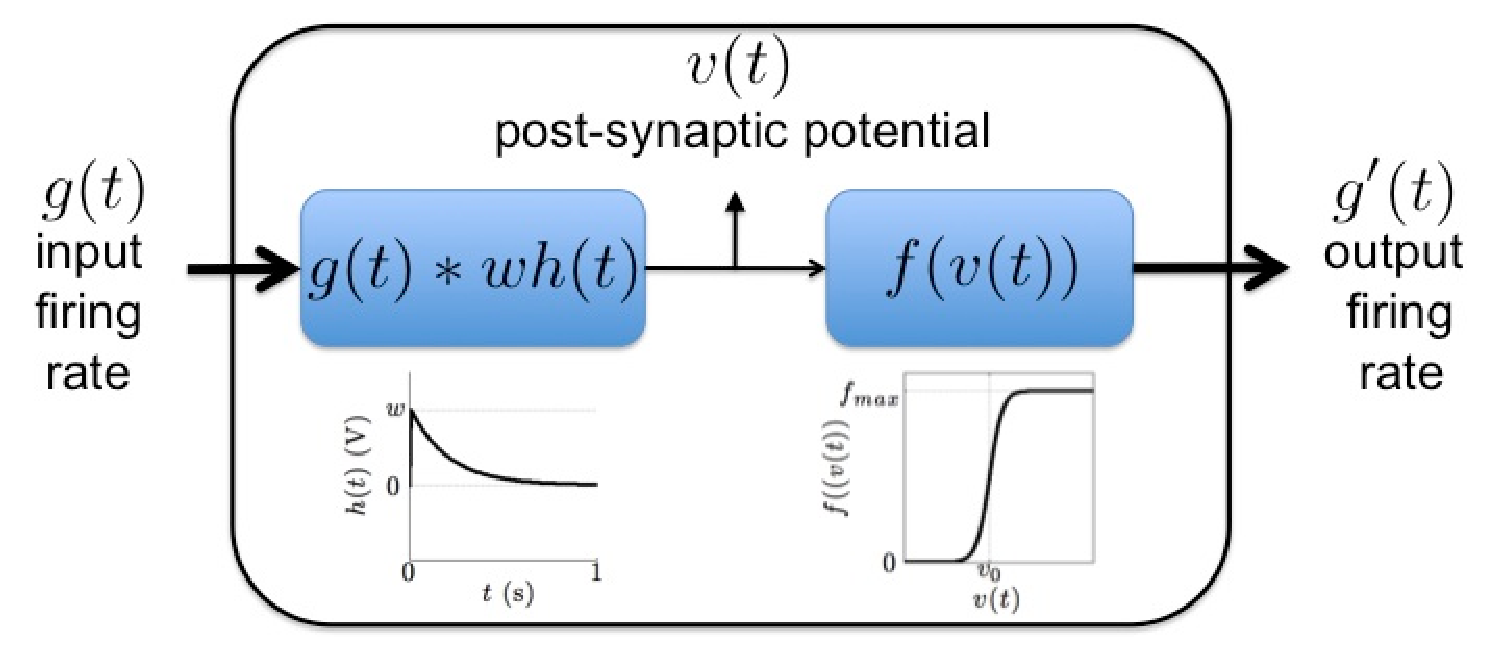
\includegraphics[width=8in, scale = 10]{FieldModel.eps}
	\end{center}
	\caption{{\bf Diagram of neural mass.} Pictorial representation of the rate-to-voltage and voltage-to-rate equations.} 
	\label{fig:Figure1}
	\end{figure}
	
    \end{column}

    \begin{column}{\sepwid}\end{column}			% empty spacer column
	
    \begin{column}{\onecolwid}					  
      

		% \setbeamercolor{block title}{fg=red,bg=white}%frame color
        \setbeamercolor{block body}{fg=black,bg=white}%body color

\begin{block}{State-Space Model}
	\begin{figure}	
	\begin{center}
	  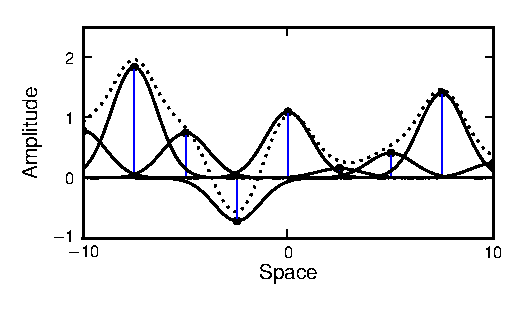
\includegraphics[width=8in, scale = 10]{Figure2.eps}
	\end{center}
	\caption{{\bf Example of a one-dimensional field decomposition.} The dashed line depicts the field, the black solid lines shows the Gaussian basis functions and the vertical lines show the position and amplitude of the states.} 
	\label{fig:Figure2}	
	\end{figure}
	\rmfamily{To implement standard estimation techniques, we use a set of Gaussian basis functions to decompose the field \cite{Dewar2009}. The field decomposition is described by 
	\begin{equation}
		\label{DefFieldDecomp} v_t\left(\mathbf{r}\right) \approx \boldsymbol{\phi}^{\top}\left(\mathbf{r}\right) \mathbf{x}_t, 
	\end{equation}
	where $\mathbf{x}_t$ is the state vector that scales the field basis functions $\mathbf{\boldsymbol{\phi}}(\mathbf{r})$. 
	The connectivity kernel can also be decomposed as 
	\begin{equation}\label{DefKernelDecomp}
		 w\left(\mathbf{r},\mathbf{r}'\right) =\boldsymbol{\psi}^\top\left(\mathbf{r},\mathbf{r}'\right) \boldsymbol{\theta},
	\end{equation}
	where $\boldsymbol{\psi}(\mathbf{r},\mathbf{r}')$ is a vector of Gaussian basis functions and $\boldsymbol{\theta}$ is a vector of scaling parameters. Now defining the matrices
	\begin{align}
		\boldsymbol{\Gamma} &\triangleq \int_\Omega {\boldsymbol{\phi} \left(\mathbf{r}\right)\boldsymbol{\phi} ^{\top}\left(\mathbf{r}\right)\textrm{d}\mathbf{r}} \label{eq:DefGamma} \\ 
		\boldsymbol{\Psi}(\mathbf{r}') &\triangleq T_s\boldsymbol{\Gamma}^{-1}\int_\Omega {\boldsymbol{\phi}(\mathbf{r})\boldsymbol{\psi}^{\top}\label{eq:DefPsi} (\mathbf{r}'-\mathbf{r})\textrm{d}\mathbf{r}},
	\end{align}
	where $\Gamma$ is a $L\times L$ matrix and $\Psi$ is $L \times n_{\theta}$ matrix, where $L$ is the number of basis functions (states) and $n_{\theta}$ is the number of connectivity kernel basis functions. The state disturbance is defined as
	\begin{equation}\label{eq:Wt} 
		\mathbf{e}_t \triangleq \boldsymbol{\Gamma}^{-1}\int_\Omega {\boldsymbol{\phi} ( \mathbf{r} )e_t( \mathbf{r} )\textrm{d}\mathbf{r}},
	\end{equation}
	which is a zero mean normally distributed white noise process with covariance
	\begin{equation}
		\boldsymbol\Sigma_e =\mathbf{\Gamma}^{-1}\int_{\Omega}\int_{\Omega}\boldsymbol{\phi}\left(\mathbf r\right) \gamma\left(\mathbf r- \mathbf r' \right)\boldsymbol{\phi}\left(\mathbf r'\right)^{\top}d\mathbf r' d\mathbf r\mathbf{\Gamma}^{- \top}. 
	\end{equation}
	By rearranging Eq.~\ref{DiscreteTimeModel} and substituting in Eqs. \ref{DefFieldDecomp}, \ref{eq:FieldBasisFunction}, \ref{eq:DefGamma}, \ref{eq:DefPsi} and \ref{eq:Wt} we get the following state-space model
	\begin{alertblock}{State-Space Model}
	\begin{align}
		\mathbf{x}_{t+1} &= \int_\Omega \boldsymbol{\Psi}(\mathbf{r}') f(\boldsymbol{\phi}^{\top}(\mathbf{r}')\mathbf{x}_t) \textrm{d}\mathbf{r}' \boldsymbol{\theta} + \xi\mathbf{x}_t + \mathbf{e}_t \\
		\mathbf{y}_t &= \mathbf{C}\mathbf{x}_t + \boldsymbol{\varepsilon}_t.
		\end{align} 	
	\end{alertblock}
	where the observation matrix is 
	\begin{equation}
			\mathbf{C} = \left[
			\begin{array}{{ccc}} 
				c_{1,1} & \dots & c_{1,L} \\
				\vdots & \ddots & \vdots \\
				c_{N,1} & \dots & c_{N,L} 
			\end{array}
			\right] 
		\end{equation}
		and 
		\begin{equation}
			c_{i,j} = \int_{\Omega}m(\mathbf{r}_i - \mathbf{r}')\boldsymbol{\phi}_j(\mathbf{r}')\textrm{d}\mathbf{r}'. 
		\end{equation}
	}
\end{block}

    \end{column}



  \begin{column}{\sepwid}\end{column}			% empty spacer column
	\begin{column}{\onecolwid}

					  
      \begin{block}{Frequency Analysis}
		\begin{figure}
		\begin{center}
		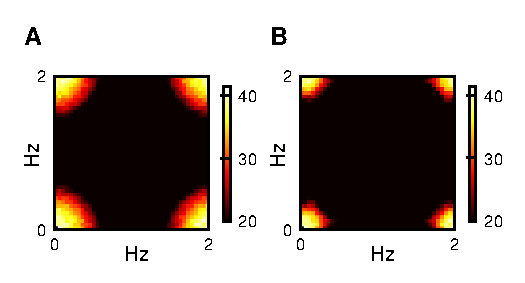
\includegraphics[width=8in, scale = 10]{Figure4.eps}
		\end{center}
		\caption{{\bf Spatial frequency analysis of the neural field}. (\textbf{A}) The average (over time) power in dB of the spatial frequency of the neural field. (\textbf{B}) The average (over time) power in dB of the spatial frequency of the reconstructed neural field from the basis function decomposition.}
		\label{fig:Figure4}
		\end{figure}
		\rmfamily{Given a band-limited field, the distance between adjacent sensors, $\Delta_y$, must satisfy 
		\begin{equation}
			\label{eq:MinimumSensorDistance} \Delta_y \leq \frac{1}{2\rho_y\boldsymbol{\nu}_{c}}, 
		\end{equation}
		where $\rho_y \in \mathbb{R} \ge 1$ is an oversampling parameter and $\boldsymbol{\nu}_c$ is a cutoff frequency (typically taken as the -3~dB point). This condition must be satisfied to avoid spatial spectral aliasing effects when reconstructing the hidden dynamic field, $v_t(\mathbf{r})$, using the sampled observations, $\mathbf{y}_t$.
		
		In the same manner the minimum distance between basis functions must satisfy 
		\begin{equation}\label{eq:BasisFunctionSeparation}
			\Delta_{\phi} \leq \frac{1}{2\rho_{\phi}\boldsymbol{\nu}_{cy}}
		\end{equation}
		where $\rho_{\phi} \in \mathbb{R} \ge 1$ is an oversampling parameter to determine the basis function separation and $\boldsymbol{\nu}_{cy}$ is the cut-off frequency of the observed field.
		The field basis function widths can also be inferred using spectral considerations~\cite{Scerri2009}. The basis function width, $\sigma^2_{\phi}$, should be chosen to be
		\begin{equation}\label{eq:WidthCutOffRelationship}
		 \sigma^2_{\phi}= \frac{1}{\pi^2\sigma_{\nu_{cy}}^2},
		\end{equation}
		where
		\begin{equation}\label{eq:WidthFrequencyRelationship}
		 \sigma^2_{\nu_{cy}}= \frac{2\boldsymbol\nu_{cy}^\top \boldsymbol\nu_{cy}}{\ln2}.
		\end{equation}}
	\end{block}
	% \vskip2ex
	\begin{block}{Estimation}
		\rmfamily{The estimation procedure consists of a two-stage iterative algorithm incorporating the unscented Rauch-Tung-Striebel smoother for state estimation and a least squares algorithm for parameter estimation.} 
	\end{block}	
	\begin{block}{References}
        \small{\rmfamily{\begin{thebibliography}{99}
\bibitem{Deco2008} G. Deco, V. Jirsa, P. Robinson, M. Breakspear, K. Friston. PLoS Computational Biology. \textbf{4} (2008).
\bibitem{Dewar2009} M. Dewar, K. Scerri, V. Kadirkamanathan. IEEE Transactions on Signal Processing. \textbf{57} (2009) 83-91.
\bibitem{Scerri2009} K. Scerri, M. Dewar, V. Kadirkamanathan. IEEE Trans. on Signal Processing. \textbf{57} (2009) 482-492.
        \end{thebibliography}}}	\end{block}
\end{column}

  \begin{column}{\sepwid}\end{column}			% empty spacer column
	\begin{column}{\onecolwid}	

      			  
      \begin{block}{Results}
		\begin{figure}	
		\begin{center}
		  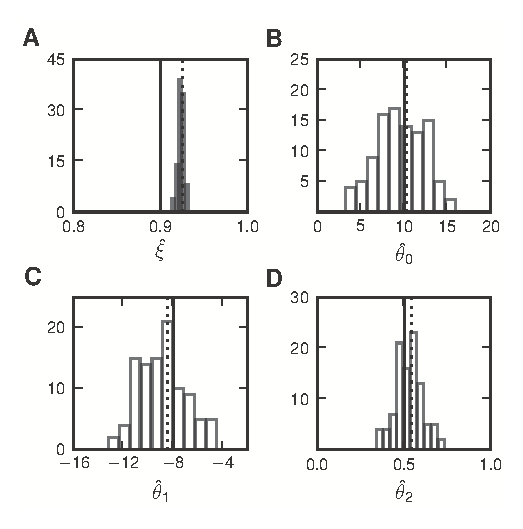
\includegraphics[width=8in, scale = 10]{Figure7.eps}
		\end{center}
		\caption{{\bf Histograms of the parameter estimates over 100
		realisations}. Solid lines show the actual parameters and the dotted lines show the means of estimated parameters. (\textbf{A}) The synaptic time constant. (\textbf{B}) The central excitatory connectivity parameter. (\textbf{C}) The surround inhibition connectivity parameter. (\textbf{D}) The longer range excitatory connectivity parameter.} 
		\label{fig:Figure7}	
		\end{figure}
		\begin{figure}
		\begin{center}
		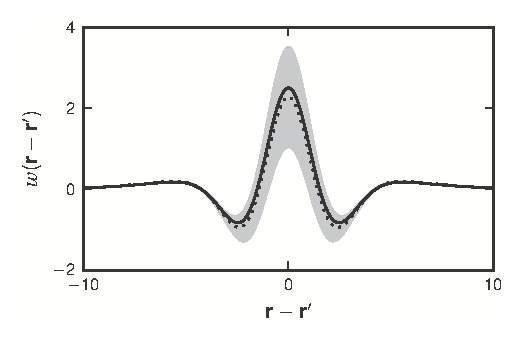
\includegraphics[width=8in, scale = 10]{Figure8.eps}
		\end{center}
		\caption{{\bf Cross-section of connectivity kernel estimate}. The actual kernel is shown by the solid line, the mean kernel estimate (over 100 realisations) is shown by the dotted line and the 95~\% confidence interval is shown by the shaded grey region.}
		\label{fig:Figure8}
		\end{figure}
				
		\begin{figure}
		\begin{center}
		\includegraphics[width=10.5in, scale = 10]{FieldComparison.eps}
		\end{center}
		\caption{{\bf Examples of the actual and estimated neural fields and the error}. (\textbf{A}) The actual field at a single time instant from the full neural field model that was used to generate the data. (\textbf{B}) The reconstructed field of the reduced model, showing the effect of the basis function decomposition on the frequency content of the estimated field.}
		\label{fig:Figure10}
		\end{figure}
		
	\end{block}
\end{column}

	\begin{column}{\sepwid}\end{column}			% empty spacer column

 \end{columns}
\end{frame}
\end{document}
